\section{Introduction}\label{sec:introduction}

Great introductions here~\cite{CERN-LHCC-2022-005,nanobind}.

\begin{figure}
    \centering
    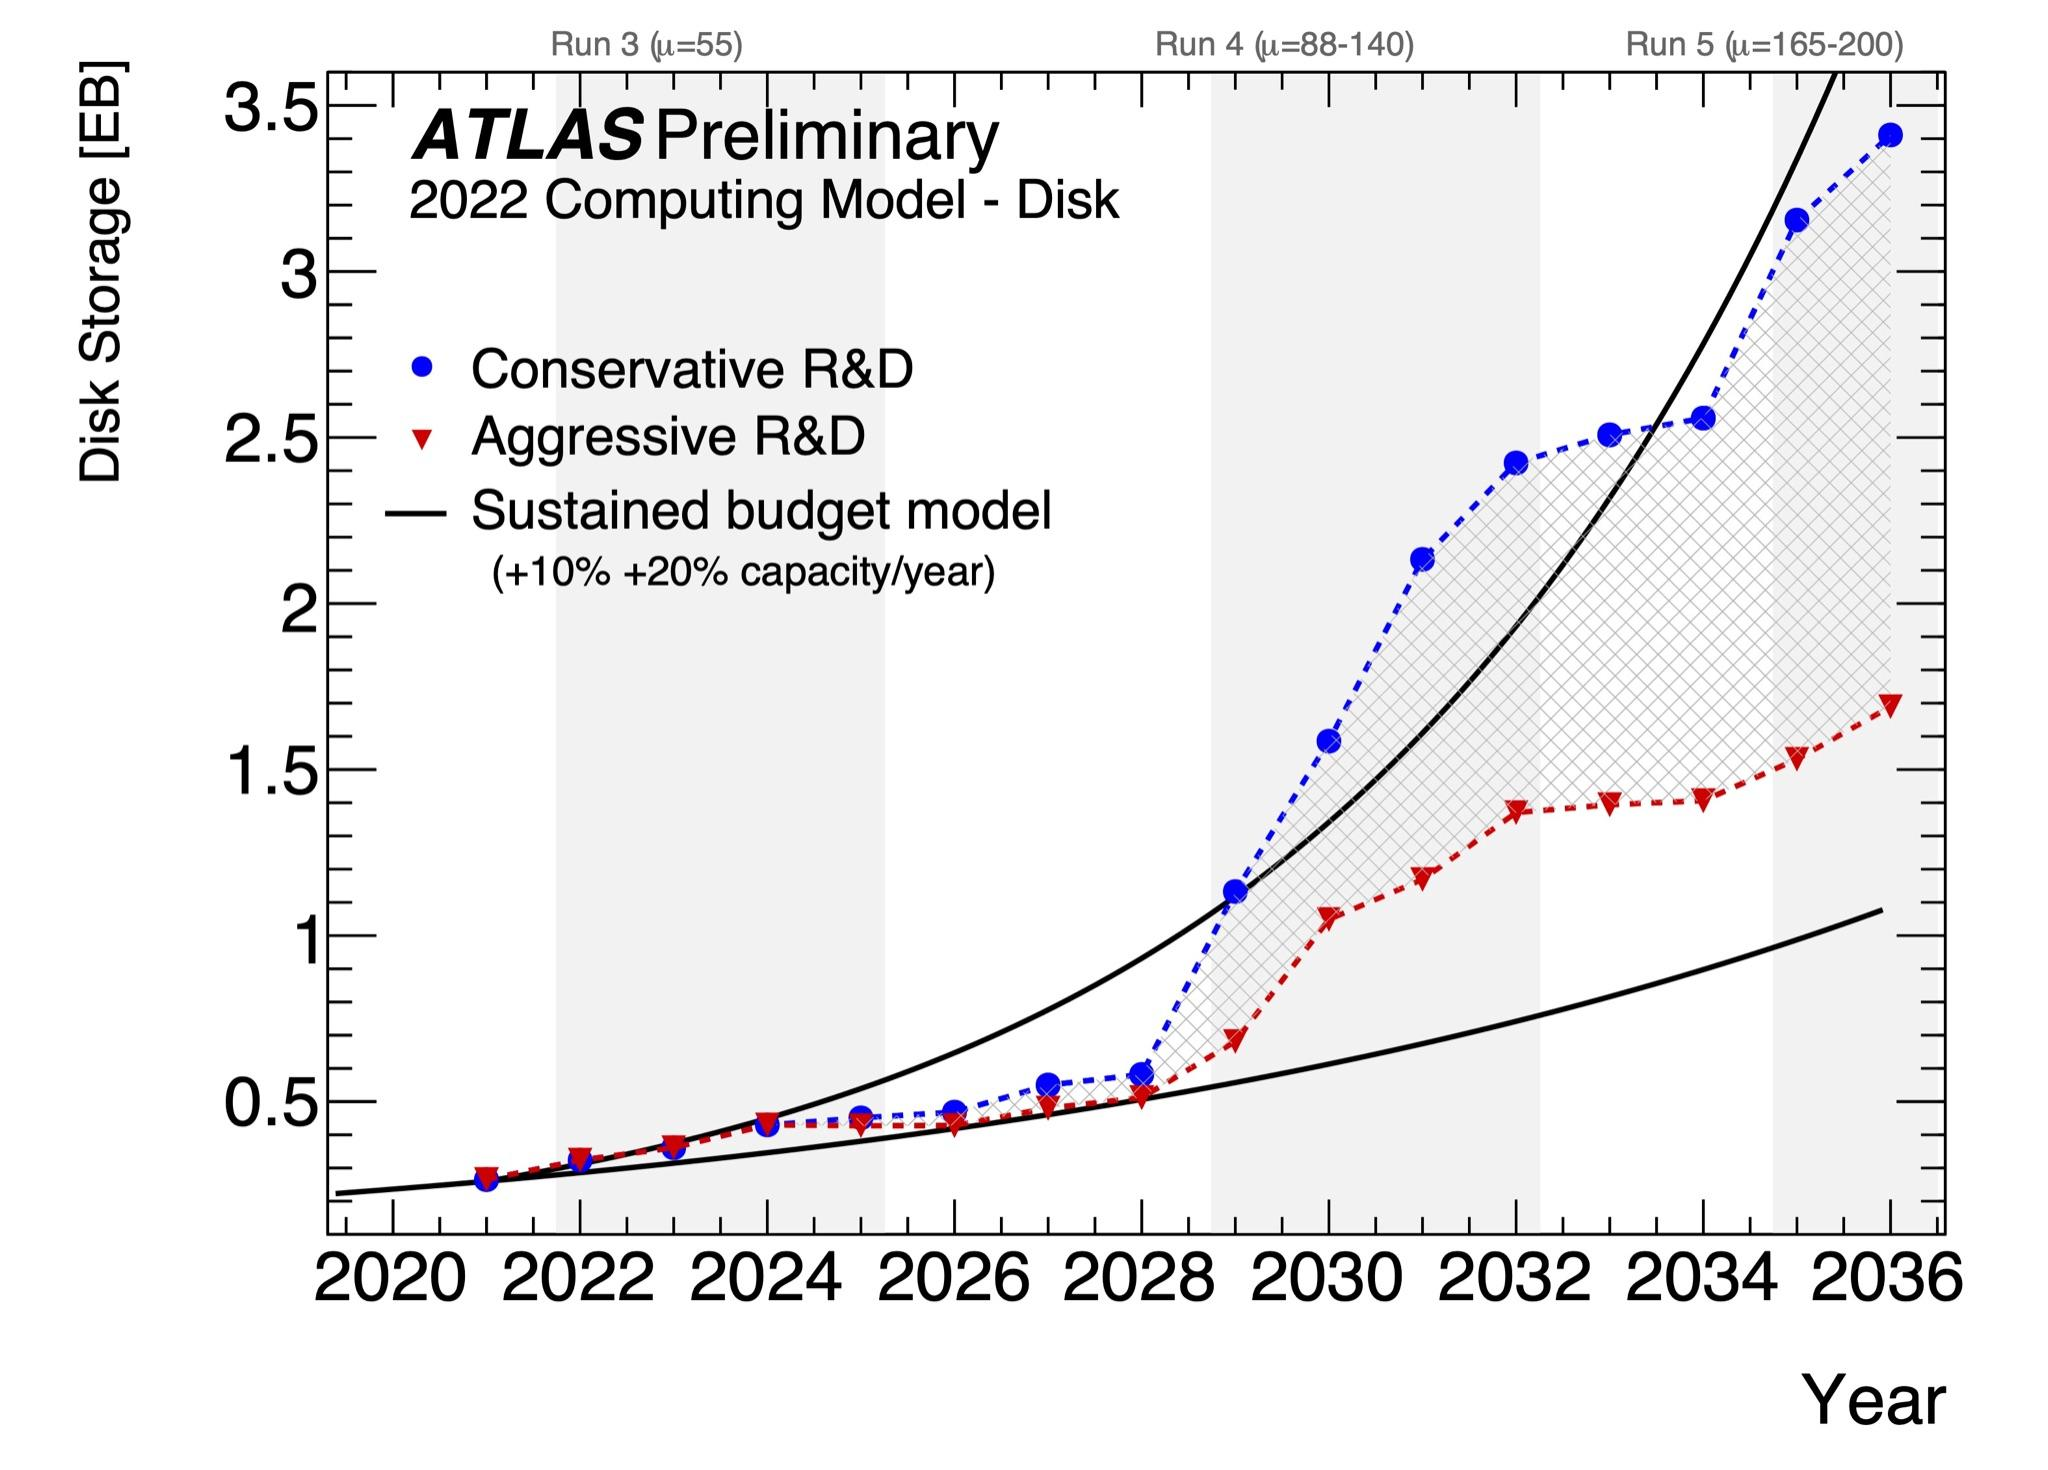
\includegraphics[width=0.8\textwidth]{atlas-disk-projection.png}
    \caption{Projected evolution of disk usage from 2020 until 2036, under the conservative (blue) and aggressive (red) R\&D scenarios.
The grey hatched shading between the red and blue lines illustrates the range of resources consumption if the aggressive scenario is only partially achieved.
The black lines indicate the impact of sustained year-on-year budget increases, and improvements in new hardware, that together amount to a capacity increase of 10\% (lower line) and 20\% (upper line).
The vertical shaded bands indicate periods during which ATLAS will be taking data.~\cite{CERN-LHCC-2022-005}}
    \label{fig:atlas-disk-projection}
\end{figure}
